\section{Υλοποίηση στον Καθρέφτη}
\label{sec:exercisor_mirror}
Στο Σχήμα \ref{fig:exercisor_mirror} φαίνεται η λειτουργία του Exercisor όπως έχει μεταφερθεί στον φυσικό καθρέφτη, ενώ στο Σχήμα \ref{fig:editor} διακρίνεται η λειτουργία επεξεργασίας μιας άσκησης.

\begin{figure}[h]
	\centering
	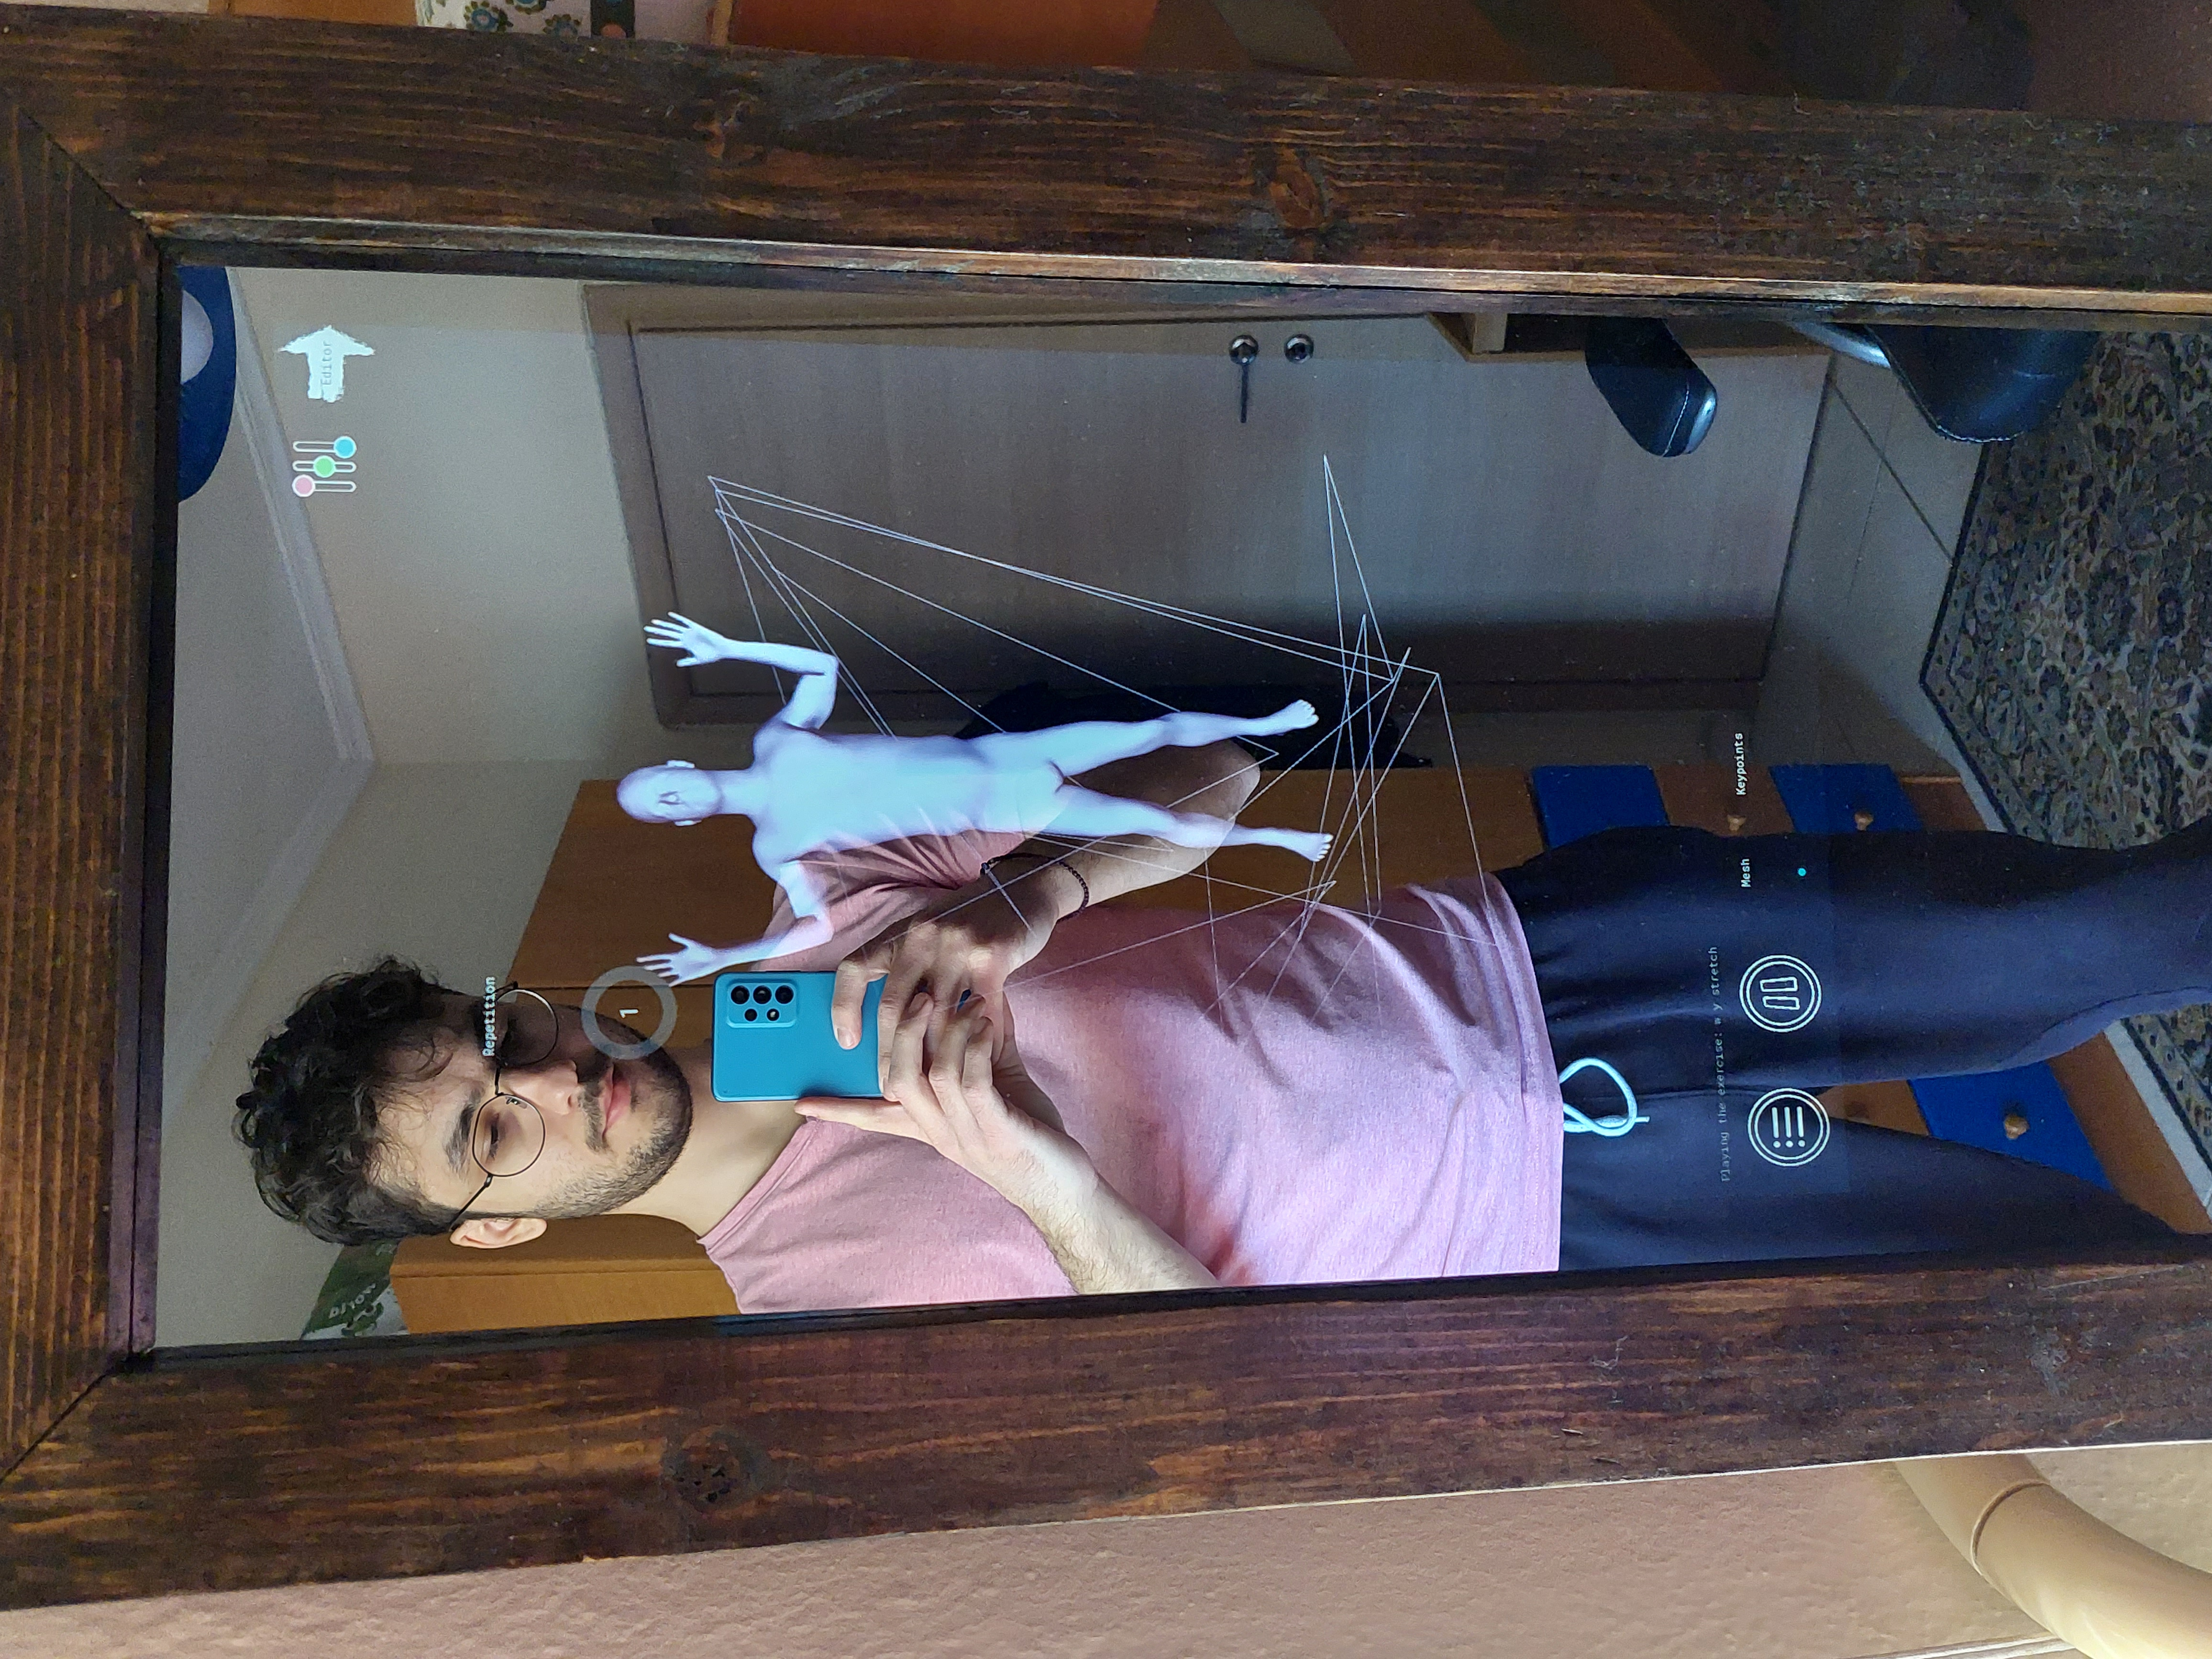
\includegraphics[scale=0.08,angle=270]{images/chapter5/exercisor_mirror.jpg}
	\caption{Μεταφορά του Exercisor στον φυσικό καθρέφτη}
	\label{fig:exercisor_mirror}
\end{figure}

\begin{figure}[H]
	\centering
	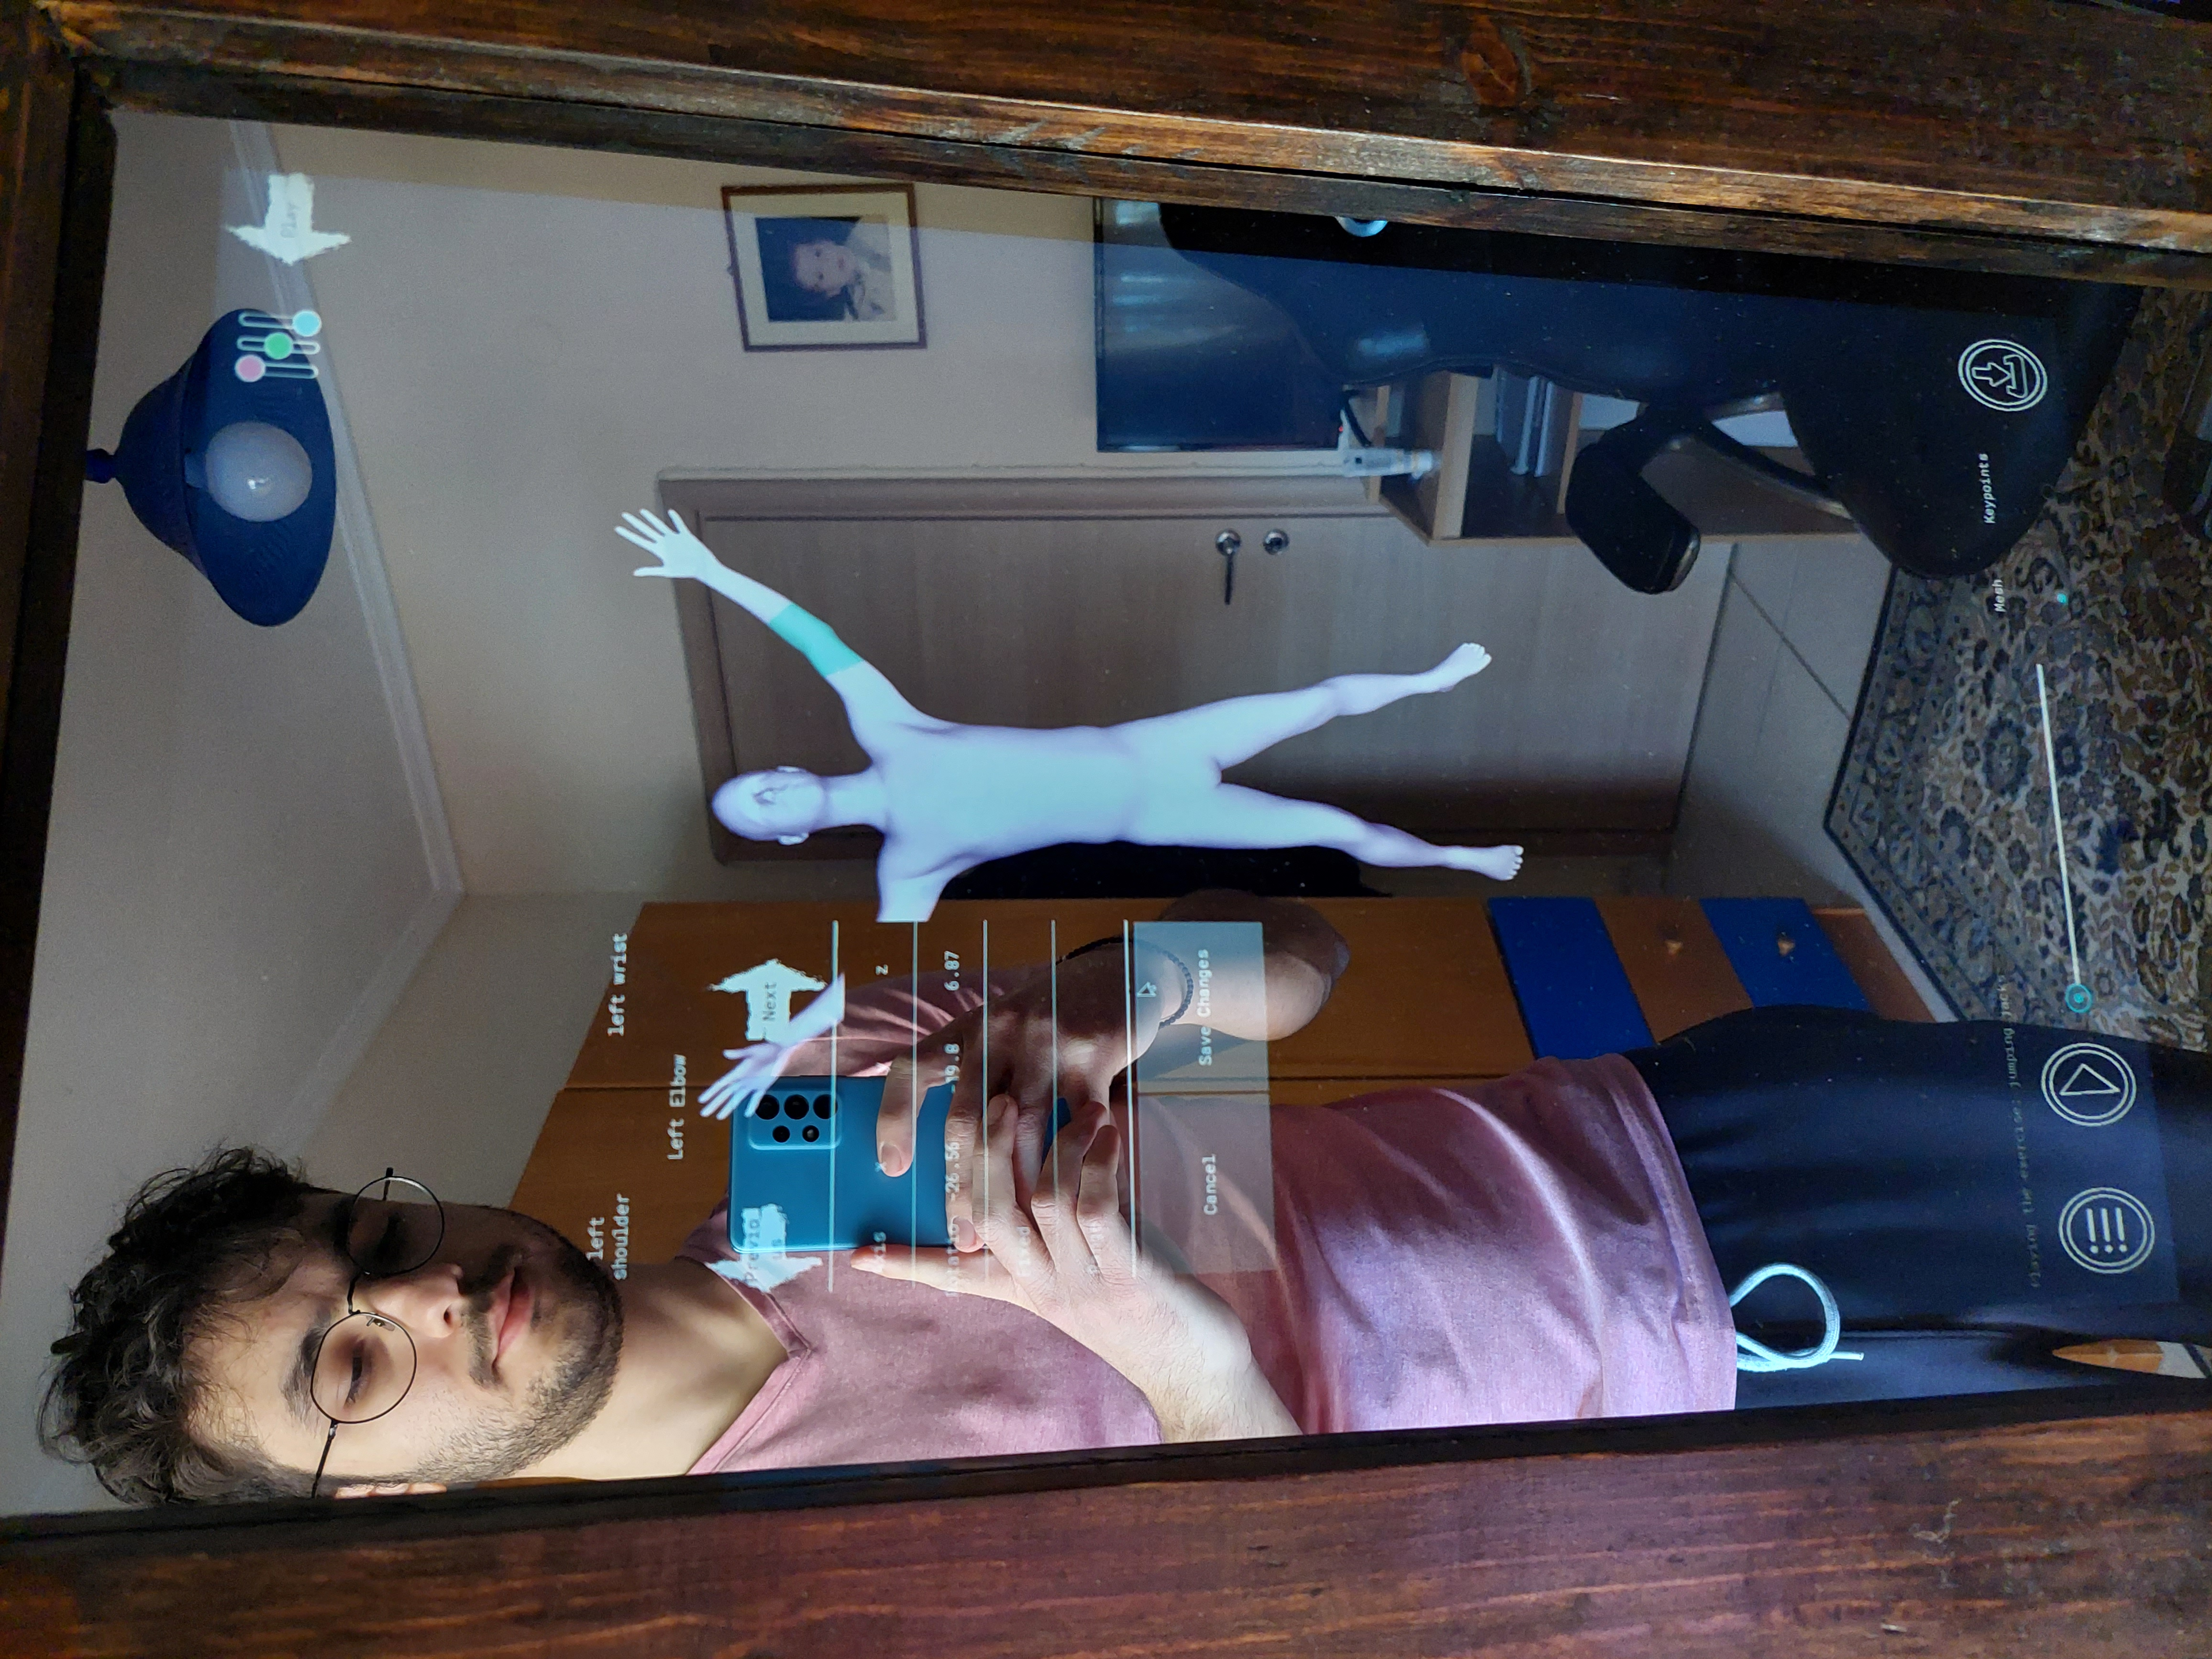
\includegraphics[scale=0.08,angle=270]{images/chapter5/editor_mirror.jpg}
	\caption{Μεταφορά του Editor στον φυσικό καθρέφτη}
	\label{fig:editor}
\end{figure}
